\chapter{Time-memory-data tradeoff using Rainbow table}
\label{chapter:tmdto-rainbow}

\paragraph{Summary}


\section{Rainbow table for block ciphers}
\label{sec:rainbow-block}

Rainbow table was introduced by Philippe Oechslin in \cite{oechslin:mfc}. Rainbow table (or rainbow chains, as called by the author) is a different way of precomputing data for the attack phase of a TMTO attack. Oechslin introduced rainbow table for block ciphers as an improvement over the Hellman tables. By using rainbow table, the attack time is expected to be reduced by a factor of $2$.

In Hellman tables, merging of chains within different tables is prevented by using different reduction functions for each table. However, collisions within the same table cannot be avoided completely. Though the number of elements in each table is restricted according to the table stopping rule, still there is no guarantee that collisions would not occur in the same table. This is due to the simple fact that birthday paradox is probabilistic in nature. Rainbow table solves this problem of collisions considerably.\\

\noindent \textit{\textbf{Precomputation phase.}} The rainbow table comprises of one huge table instead of $t$ tables, with $mt$ chains each having $t$ keys. The more interesting difference from Hellman tables is that instead of changing reduction function with table, reduction function is changed between columns in the rainbow table. If $SP_i$ is the starting point of a chain, then subsequent keys are computed by the functions \mbox{$f_1, f_2, \cdots, f_t$}, where $f_j(K) = R_j(E_{K}(P))$ for $1 \leq j \leq t$. This is shown in the following equations. 

\begin{align*}
& & K_{i,0} & = SP_i & & & &\\
1&. &K_{i,1} & = f_1(K_{i,0}) & & & &\\
2&. &K_{i,2} & = f_2(K_{i,1}) & & & &\\
& & &\vdots & & & &\\
(t-1)&. &K_{i,t-1} & = f_{t-1}(K_{i,t-2}) & & & &\\
(t)&. &K_{i,t} & = f_t(K_{i,t-1}) & & & &\\
& & EP_i & = K_{i,t} & & & &\\
\end{align*}

For every chain, the same sequence of mapping functions from $f_1$ to $f_t$ are used in computing subsequent keys. As usual, the starting and end points for each chain are stored in a hashtable, with the end points as the hashkey and the starting points as the hashvalue. The rainbow table is shown in figure \ref{fig:rainbow-table}.

\begin{figure}[ht!]
	\centering
		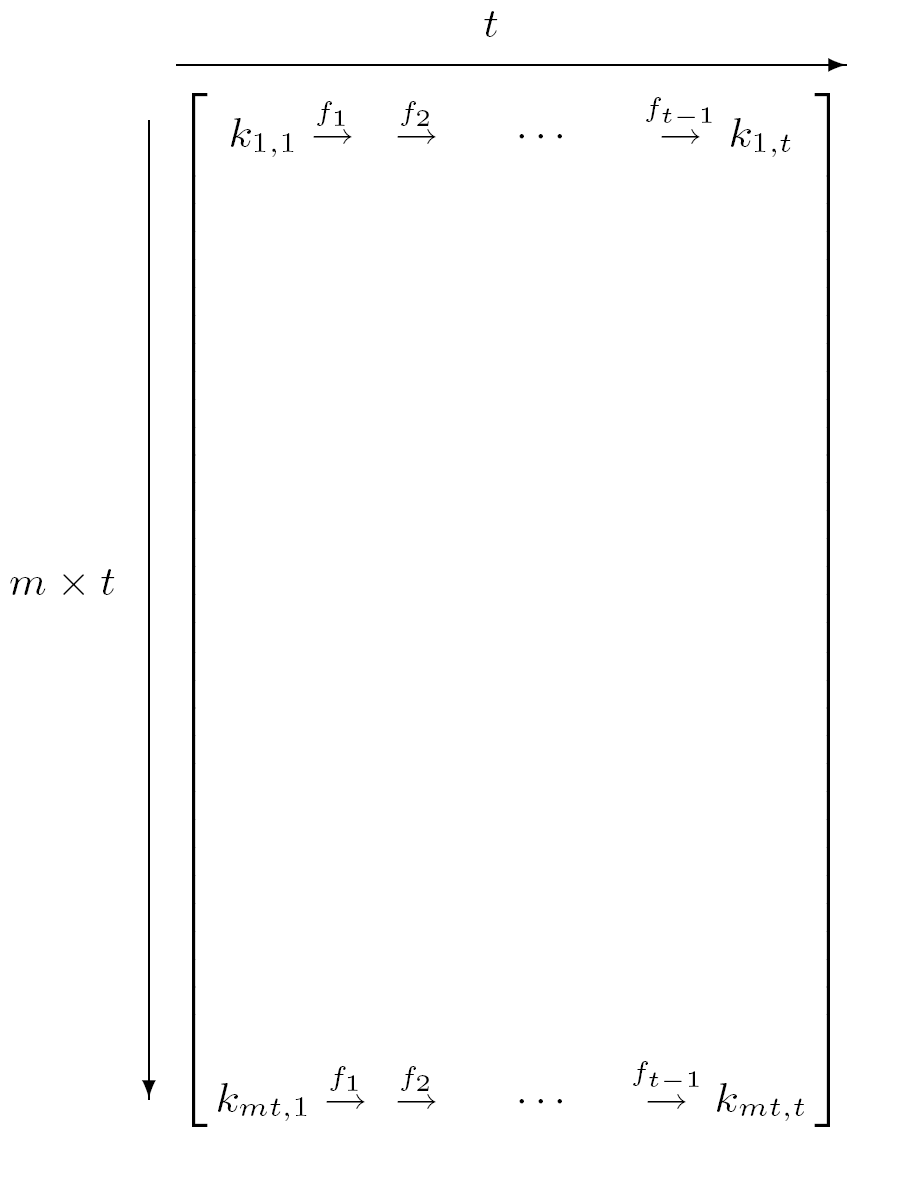
\includegraphics[width=3.5in]{./figures/rainbow-table.PNG}
	\caption{Rainbow table for block ciphers}	
	\label{fig:rainbow-table}
\end{figure}

The time for preparing the rainbow table is the same as the number of computations carried out. This is equal to $P$ = $mt \times t$ = $mt^2$. Also, the order of memory required for the hash table is $M$ = $mt$. \\

\noindent \textit{\textbf{Attack phase.}} The attack phase is a little more complicated as compared to that for Hellman tables. But, as we shall see, the number of computations required in the worst case, to find a match, is reduced by a factor of $2$. 

First, let's consider the possibility of the ciphertext appearing in the last column of the rainbow table. If this is the case, then an end point $EP_i$ would match with the reduction of the ciphertext $C$ which is $X$ = $R_t(C)$. Note that the reduction function for the $t$'th column is used here. If the match occurs, then $(t-1)$ computations are performed starting from the corresponding starting point $SP_i$, with the mapping function changing in each column. $K_{i,t-1}$ is then the required key, if it is not a false alarm. If the match does not occur, the number of operations (number of calls to any of the mapping functions $F_1$ to $F_t$) performed is $0$. 

So next, the possibility of $C$ appearing in the $(t-1)$'th column is explored. For this the value $X = F_{t}(R_{t-1}(C))$ is compared with the end points. If there is a match, then $(t-2)$ computations are performed from $SP_{i}$ using the mapping functions $F_1, F_2, \cdots, F_{t-2}$. The key $K_{i,t-2}$ computed is the required key. Otherwise, if there is no match, the number of operations performed is $1$.

This procedure is repeated for all the columns, until in a worst case scenario, $C$ happens to appear in the second column of the table. In such a case, we would iteratively call the mapping functions $F_2, F_3, \cdots, F_t$, thus amounting to $(t-1)$ operations, before $EP_j$ is matched. The total number of operations in the worst case scenario become, 

\begin{align*}
&= 0 + 1 + 2 + \cdots + (t-1)\\
&= t(t-1)/2\\
\end{align*}

\begin{align}
\label{eq:time-rainbow-single-prefix} &\approx t^2/2
\end{align}

The attack time then is of the order of $t^2/2$, thus $T$ = $t^2/2$.\\


\noindent \textit{\textbf{Tradeoff equation.}} Using the following equations, the tradeoff equation can be derived. 

\begin{align*}
M &= mt\\
T &= t^2/2\\
mt^2 &= N\\
\end{align*}

The tradeoff equation then comes to be,

\begin{align}
\label{eq:tmdto-rainbow-block} 2TM^2 &= N^2
\end{align}


\section{Rainbow table for stream ciphers and implementation}
\label{sec:rainbow-stream}

We derive a general tradeoff equation for attacks on stream ciphers using the rainbow table. An analysis similar to that done by Biryukov and Shamir for Hellman tables is described in section \ref{sec:compare-hellman-rainbow}. 

The number of chains in the rainbow table is $M$ and $t$ states exist in each chain. The total number of states in the table is $P = Mt$. Also, $D$ states occur during the attack phase. Then, again according to equation \ref{eq:bday-paradox2}, the product of $P$ and $D$ must satisfy the relation $P \times D \geq N$. Considering the lower bound for $P$ and $D$, we have $P \times D = N$ giving us the general tradeoff equation as follows.

\begin{align}
\label{eq:general-rainbow-stream} Mt \times D = N
\end{align}
 
This relation allows us to select the parameters $M$, $t$ and $D$ in a manner such that the precomputation phase and the attack phase can be carried out without any dependencies on each other. The attack phase runs in the same way as for block ciphers. The time for searching a prefix in the hashtable is $t^2/2$, as from equation \ref{eq:time-rainbow-single-prefix}. Hence, the total attack time for $D$ match attempts is $T = t^2D/2$. \\

\noindent \textbf{\textit{Implementation}}. Since there is just one table storing all the states, only one hashtable is required for storing the starting and end point of each chain. Similar to the precomputation phase using Hellman tables, we have implemented a separate program which computes the rainbow table and stores it on the local disk in the form of an ASCII file. The attack module reads the starting and end points from this file, and prepares the hashtable. Keystream of appropriate length depending on the value of $D$ is prepared for the attack. 

Following are the results of the attack for keys $K_1$ and $K_2$. 

\begin{table}[ht!]
\begin{center}
\begin{tabular}{|c||c|c||c|c|}
\hline
Key & \multicolumn{2}{c||}{\textbf{$K_1$}} & \multicolumn{2}{c|}{\textbf{$K_2$}} \\ \hline \hline
M																				&	$2^{24}$ 	&	$2^{24}$ 	&	$2^{24}$ 	&	$2^{24}$ 	\\ 
t	  																		&	$2^{8}$ 	&	$2^{9}$ 	&	$2^{8}$ 	&	$2^{9}$		\\ 
D	  																		&	$2^{16}$ 	&	$2^{15}$ 	&	$2^{16}$ 	&	$2^{15}$	\\ \hline \hline
P	  																		&	$2^{32}$ 	&	$2^{33}$ 	&	$2^{32}$ 	&	$2^{33}$	\\ \hline
T	  																		&	$2^{31}$ 	&	$2^{32}$ 	&	$2^{31}$ 	&	$2^{32}$	\\ \hline
Precomputation time for file (hours)		&	6 	 			&	12 				&	6					&	12 				\\ \hline
Time for preparing hashtable (seconds)	&	158				&	102				& 116				&	116				\\ \hline
Number of times false key is found			&	2 				&	1 				&	3 				&	3 				\\ \hline
Number of times correct key is found 		&	2 				&	3					&	3 				&	1 				\\ \hline
Number of false alarms									&	139				&	245				&	120				&	256				\\ \hline
Time for attack	(hours)									&	2.25 			&	5.10			&	2.56 		 	&	5.12 			\\ \hline
\end{tabular}
\end{center}
\caption{Results of TMDTO rainbow attack for keys $K_1$ and $K_2$}
\label{tab:rainbow-attack-results}
\end{table}

The following comments can be made based on the results from table \ref{tab:rainbow-attack-results}.
\begin{enumerate}
\item The time taken in creating the rainbow table (precomputation time for file) depends on $P$ or the number of states stored in the table. For $P$ = $2^{31}$, the time taken is around 6 hours, while for $P$ = $2^{32}$ it takes around 12 hours. 

\item The time for preparing the hashtable must be the same for all the cases (and both the keys), since $M$ is the same. But, we notice certain irregularity in the time, and this can be attributed to the machine on which the attack is run, as it is shared between various users. 

\item The correct key is found atleast once in all the cases, which is a good sign. Though, along with correct key, wrong keys are also being found in the attack. This must not be mistaken with the false alarms. These cases arise because of a prefix having more than one generating state or preimage. As a result, the prefix correctly exists in the rainbow table but with the wrong state as its preimage. This state is found by the attack, resulting in a wrong key. We call such cases as false keys, and stress that they are different from false alarms. The only way of avoiding false keys is by increasing the length of prefix to 56 bits. As we have seen for TMTO keystream and tags attacks, 56 bits of prefix is sufficient in order to supress false keys. 

\item The time for attack is the total time taken for searching all the subsequences of the keystream. We have continued the attack even after the correct key is found, to know other results for the complete attack and the time taken for the same. For example, for the parameters in column 1 of $K_1$, the key is found for the first time in 595 seconds. The output from the attack is shown below.

\begin{lstlisting}[frame=tb]
Match!

Status:- D: 4800, Found column: 49
Found prefix: 196721643589477
Found Initial State: fe6e391b4972
Found Key: 52b49ea34972
TIME since starting attack: 595
\end{lstlisting}

It also says that the key is found in the 49'th column of the rainbow table, for the 4800'th subsequence of the keystream. 
\end{enumerate}


\section{Comparison of Hellman and rainbow table}
\label{sec:compare-hellman-rainbow}

For using Hellman tables for stream ciphers, Biryukov and Shamir proposed changes by modifying the table structure using the parameter $D$. The original idea of rainbow table has been proposed for block ciphers and thus similar modification in the table structure needs to be done to apply them on stream ciphers. The paper \cite{erguler2005nct} by Erguler and Anarim is the only work in this direction, to be best of our knowledge. It discusses an approach on similar lines of Biryukov and Shamir approach. The tradeoff described here was designed independently by us. Only later it came to our knowledge that the idea has already been published by Erguler and Anarim.

Since we have data available for stream ciphers, the number of states in the rainbow table should be reduced by a factor of $D$. The number of states existing in the rainbow table is $Mt$ \footnote{The parameters $M$ and $t$ here represent the original rainbow table, and are not related with the parameters described in the general tradeoff equation in previous section}. If they have to be reduced, then either $M$ or $t$ or both should be reduced. Three such possibilities are identified in the following table. 

\begin{table}[ht!]
\begin{center}
\begin{tabular}{|c||c||c c c|}
\hline
			& Biryukov-Shamir approach 	& \multicolumn{3}{c|}{Approach for rainbow tables}					\\ \hline \hline
M			&	M/D		&	M/D				&	M						& $M/\sqrt{D}$	\\
t			&	t			&	t					&	t/D					& $t/\sqrt{D}$	\\ \hline \hline
P			&	Mt/D	&	Mt/D			&	Mt/D				& Mt/D					\\ 
T			&	$t^2$	&	$t^2D/2$	&	$t^2/2D$		& $t^2/2$				\\ \hline
\end{tabular}
\end{center} 
\caption{Possible cases for modifying $M$ and $t$ for rainbow tables}
\label{tab:parameters-rainbow-table}
\end{table}

The first case for rainbow tables is reducing $M$ to $M/D$. Though memory required for the attack reduces, the time for the attack increases considerably to $t^2D/2$. It is interesting to note that for Hellman tables, the attack time depends on both $t$ and the number of tables. So, if $M$ is decreased, the number of tables decreases, thus reducing the attack time to $t^2$. On the other hand, for rainbow tables, the attack time depends just on $t$. Hence, reducing the memory does not reduce the time for the attack by a factor $D$.

In the next case, we reduce $t$ to $t/D$. The problem with this option is the increased memory requirement which is $M$. The third option is a middle way between the first two options. We reduce $M$ and $t$ by a factor of $\sqrt{D}$. The attack time now becomes ${(t/\sqrt{D})}^2/2 \times D$ = $t^2/2$. As we see, this makes it comparable to the attack time for Hellman tables. Rainbow tables provide the same advantage for stream ciphers in this context, as they do for block ciphers i.e. they reduce the attack time by a factor of 2. But, as can be seen, for stream ciphers the memory requirement is increased $\sqrt{D}$ times, which is a disadvantage of using rainbow tables with these parameters.

Let us denote the memory requirement and the number of states in each chain by $M'$ and $t'$ for the modified rainbow table. Then we have $M' = M/\sqrt{D}$ and $t' = t/\sqrt{D}$. Replacing these values in the general tradeoff equation \ref{eq:general-rainbow-stream}, we get the following tradeoff equation.

\begin{align}
\label{eq:tmdto-rainbow-stream} 2TM^2D^2 &= N^2
\end{align}

For comparing the performance of Hellman and rainbow tables using their tradeoff equations, we select the following values of the required parameters. 

\begin{table}[ht!]
\begin{center}
\begin{tabular}{|c|c c||c c|}
\hline
			& \multicolumn{2}{c||}{$M = 2^{32}$, $t = 2^{16}$, $D = 2^{14}$} 	& \multicolumn{2}{c|}{$M = 2^{31}$, $t = 2^{17}$, $D = 2^{16}$}	\\ \hline \hline
			&	Hellman				&	Rainbow					&	Hellman					& Rainbow				\\ \hline \hline
M			&	$2^{18}$			&	$2^{25}$				&	$2^{15}$				& $2^{23}$			\\ \hline 
m			&	$2^{16}$			&		-							&	$2^{14}$				& 	-						\\ \hline 
r			&	$2^{2}$				&		-							&	$2^{1}$					& 	-						\\ \hline 
t			&	$2^{16}$			&	$2^{9}$					&	$2^{17}$				& $2^{9}$				\\ \hline 
P			&	$2^{34}$			&	$2^{34}$				&	$2^{32}$				& $2^{32}$			\\ \hline 
T			&	$2^{32}$			&	$2^{31}$				&	$2^{34}$				& $2^{33}$			\\ \hline 
\end{tabular}
\end{center} 
\caption{Parameters for comparison of Hellman and rainbow table}
\label{tab:parameters-comparison}
\end{table}